\begin{figure*}[t]
  \centering
  \begin{subfigure}[b]{\textwidth}
  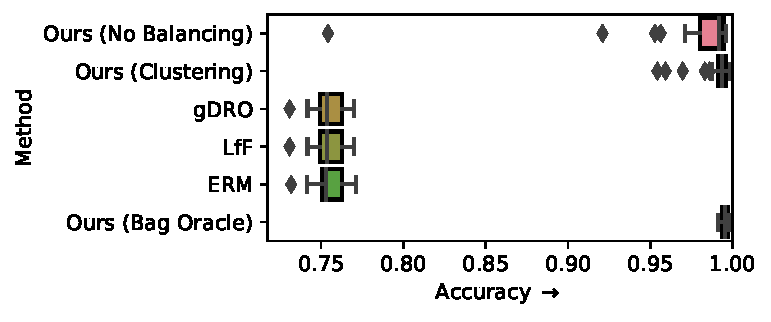
\includegraphics[width=0.49\textwidth]{supmatch/figures/cmnist/subgroup_bias/cmnist_2v4_partial_acc.pdf}
  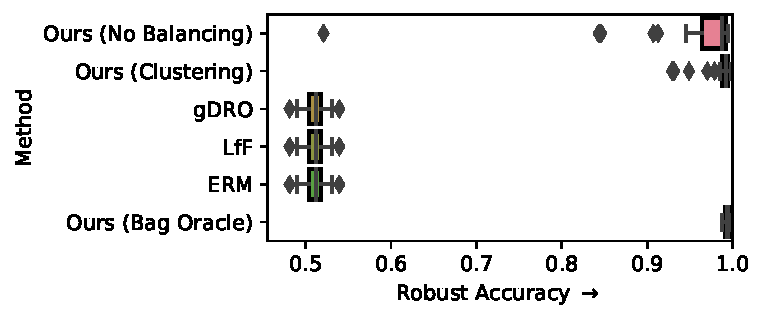
\includegraphics[width=0.49\textwidth]{supmatch/figures/cmnist/subgroup_bias/cmnist_2v4_partial_acc-min.pdf}
%   \includegraphics[width=\columnwidth]{figures/cmnist_2v4_partial_tpr.pdf}
%   \includegraphics[width=\columnwidth]{figures/cmnist_2v4_partial_tnr.pdf}
  \caption{
    Results for the \emph{subgroup-bias} scenario where {\color{purple}purple} fours constitute the missing source.
    %
    The clustering accuracy for \texttt{Ours (No Balancing)} was 96\% $\pm$ 6\%.
    %
    Our method consistently outperforms the baselines, which fare no better than random on the subgroup with the missing source. 
    %
    As we would expect, the median and IQR of our method are positively- and negative- correlated, respectively, with how well the bags of the deployment set are balanced, with \texttt{Ours (Bag Oracle)} providing an upper bound for this.
    %
    Indeed, in one case \texttt{Ours (No Clustering)} failed to surpass the baselines, but through use of clustering the \texttt{Robust Accuracy} is kept within the region of $95\%$ at worst.
  }%
  \label{fig:cmnist-2v4-partial}
% \end{figure*}
% \begin{subfigure}
  \end{subfigure}
  
  \begin{subfigure}[b]{\textwidth}
  \centering
  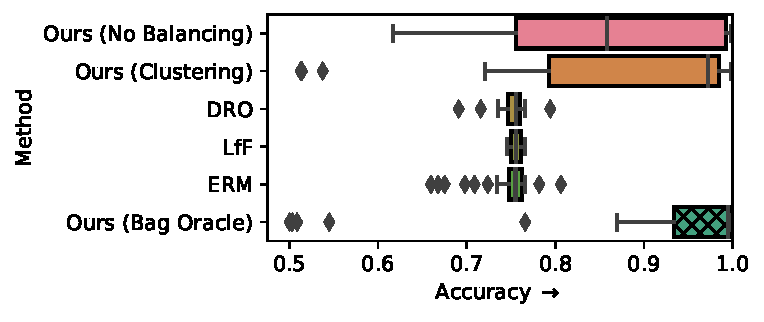
\includegraphics[width=0.49\textwidth]{supmatch/figures/cmnist/missing_subgroup/cmnist_2v4_miss_s_acc.pdf}
  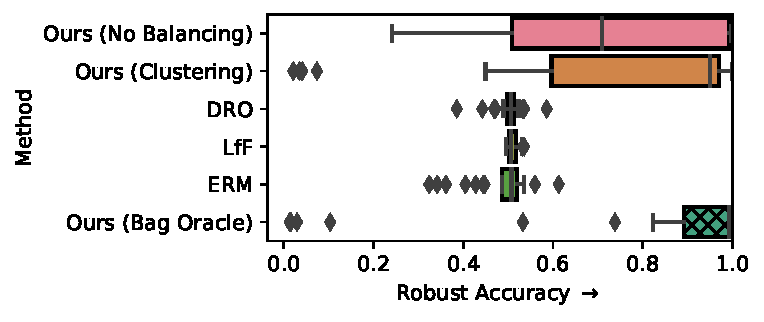
\includegraphics[width=0.49\textwidth]{supmatch/figures/cmnist/missing_subgroup/cmnist_2v4_miss_s_acc-min.pdf}
%   \includegraphics[width=\columnwidth]{supmatch/figures/cmnist_2v4_miss_s_alt_tpr.pdf}
%   \includegraphics[width=\columnwidth]{supmatch/figures/cmnist_2v4_miss_s_alt_tnr.pdf}
  \caption{
    Results for the \emph{missing-subgroup scenario} where {\color{purple}purple} digits constitute the missing subgroup.
    %
    The clustering accuracy for \texttt{Our (No Balancing)} was 88\% $\pm$ 5\%. 
    This scenario is significantly more difficult to solve than the subgroup-bias as there is insufficient inductive bias in the labels and the deployment set for the support matching to be well-posed. 
    %
    This is reflected in the high variance of our method, variance, however, which can be drastically reduced by improving the quality of balancing.
    %
    Nevertheless, all variants of our method perform significantly better than the baselines in terms of the median \texttt{Robust Accuracy}, and the rate at which they produce degenerate solutions (marked by performance worse than \texttt{ERM}'s) relatively low.
    %
  }%
  \label{fig:cmnist-2v4-miss-s}
  \end{subfigure}
  \caption{
  Results for two-digit Colored MNIST for two different scenarios (subgroup bias (Top) and missing subgroup (Bottom)) in the form of box plots of the \texttt{Robust Accuracy} (the minimum accuracy computed over the subgroups) over \textbf{30 repeats}.
  }
\end{figure*}
